% Inbuilt themes in beamer
\documentclass[aspectratio=169]{beamer}
\usepackage{graphicx}
\usepackage{amsmath}
% Theme choice:
\usetheme{CambridgeUS}

% Title page details: 
\title{Chapter 17: Oligopoly} 
\author{Discussion section 4}
\date{December 2023}

\begin{document}

% Title page
\begin{frame}
    \titlepage 
\end{frame}

\begin{frame}{Oligopolies}
    \begin{itemize}
        \item Another example of a mix of monopolies and perfect competition
        \item Now we return to perfectly substitutable products, but\dots
        \item There are only a \textit{small number} of sellers
        \item Thus, oligopolistic firms will have pricing power
    \end{itemize}
\end{frame}

\begin{frame}{Duopoly}
    Suppose McDonalds and Burger King are the only hamburger sellers (and their burgers are now identical)
    \begin{itemize}
        \item How will they make their production decision?
        \item What would the best outcome be?
        \item Will they achieve this?
    \end{itemize}
\end{frame}

\begin{frame}{Duopoly}
    McDonalds and Burger King may try and cooperate to mimic a monopoly, and each take half of the profits.

    \vspace{2mm}

    This is \textit{collusion} and makes them a \textit{cartel}.

    \vspace{2mm}

    It would also be \textit{inefficient}. (What do I mean by this?)

    \vspace{2mm}

    But...

\end{frame}


\begin{frame}{Duopoly}
    \begin{center}
        \textbf{Collusion will be difficult to maintain.}

        \vspace{5mm}

        Why?

    \end{center}
\end{frame}

\begin{frame}{Collusion}
    Why will collusion be difficult to maintain? 

    \vspace{2mm}

    Intuition: each side has an incentive to cheat \textit{a little bit}.

    \vspace{2mm}

    If one firm increases production, what happens?
\end{frame}

\begin{frame}{Collusion}
    If one firm increases production, what happens?
    \begin{itemize}
        \item Price effect: higher market Q --> lower market P (price effect)
        \item But, for that individual firm, higher Q --> more revenue (output effect)
        \item So the oligopoly will not be able to maintain the monopoly outcome
        \begin{itemize}
            \item Also will not produce at the competitive market outcome, though: P$>$ MC but less than the free market price
            \item The more firms in the oligopoly, the closer the outcome gets to the free market
        \end{itemize}
    \end{itemize}
\end{frame}

\begin{frame}{Nash equilibrium}
    \begin{itemize}
        \item This is a \textit{Nash equilibrium}: both firms are making the best decision for themselves, given the decision of the other firm
        \item Arises in a strategic setting or game, where the behavior of others influences my own behavior
        \item Form of a prisoner's dilemma
    \end{itemize}
\end{frame}

\begin{frame}{Demand curve}
    \centering
    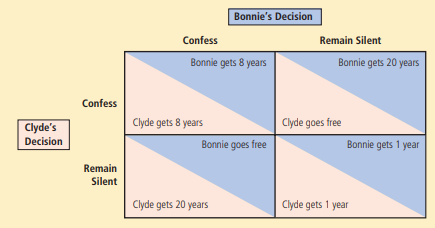
\includegraphics[width = 0.9\textwidth,keepaspectratio]{../figs/prisoners.png}
\end{frame}

\begin{frame}{Prisoners' Dilemma}
    \begin{itemize}
        \item Is this good or bad?
        \item In the case of two firms, maybe good for consumers!
        \item In the case of two super-powers, maybe bad for the world
        \item What can we do?
    \end{itemize}
\end{frame}

\begin{frame}{Prisoners' Dilemma}
    \begin{itemize}
        \item Is this good or bad?
        \item In the case of two firms, maybe good for consumers!
        \item In the case of two super-powers, maybe bad for the world
        \item What can we do?
        \begin{itemize}
            \item Threats
            \item Commitment devices
            \item Regulation
        \end{itemize}
    \end{itemize}
\end{frame}

\begin{frame}{Other anti-competitive prices}
    \begin{itemize}
        \item Tying: two goods are sold as a bundle
        \item Resale price maintenance: force your customers to resell at a certain level
        \item Predatory pricing: undercut the competition
    \end{itemize}
    As usual, Mankiw's view will be that none of these are necessarily bad.
\end{frame}

\end{document}